The following Data Flow Diagrams represent the internal functionality of the Evaluation Component.

\subsection*{Admin Interaction}

The system administrator will have the opportunity to interact with our component through a command line interface to inspect the logged search history as well as the performance metrics.

\begin{center}
  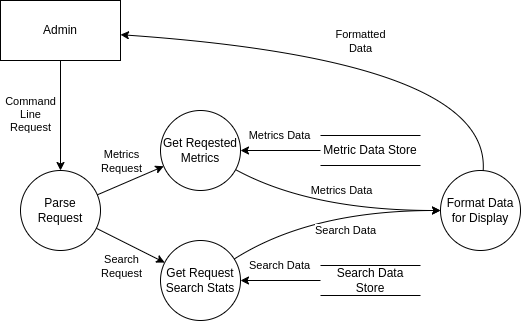
\includegraphics[scale=0.7]{DFDs/LowLevelDFDs-AdminView.drawio.png}
\end{center}

\subsection*{Get Autofill}

The UI/UX component will request autofill suggestions based on search history as described above.

\begin{center}
  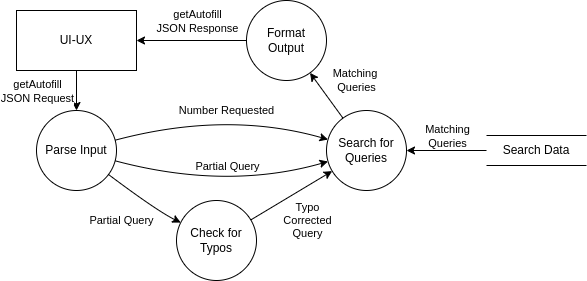
\includegraphics[scale=0.7]{DFDs/LowLevelDFDs-GetAutofill.drawio.png}
\end{center}

\subsection*{Report Metrics}

All other components will need to report metrics to the Evaluation component to monitor system performance.

\begin{center}
  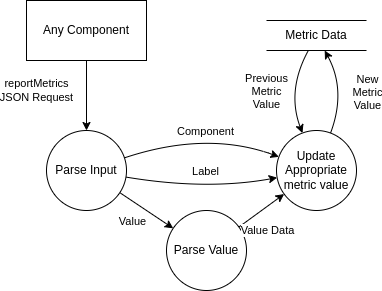
\includegraphics[scale=0.7]{DFDs/LowLevelDFDs-ReportMetric.drawio.png}
\end{center}

\subsection*{ReportSearchResults}

The UI/UX component will send all relevant information to each search interaction by the user. Subsets of this will be forwarded to the Ranking and Link Analysis teams for their use, and all information will be recorded and kept by us, the Evaluation component.

\begin{center}
  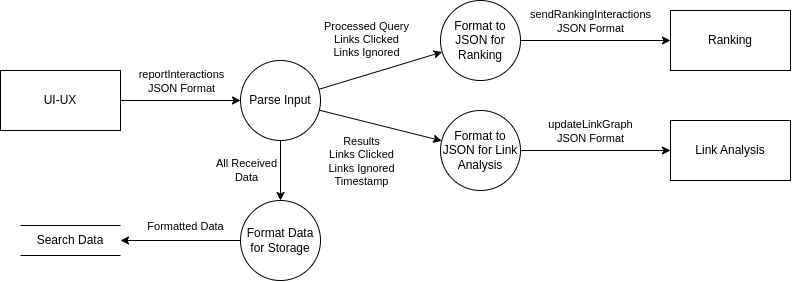
\includegraphics[scale=0.55]{DFDs/LowLevelDFDs-ReportSearchResults.drawio.png}
\end{center}